\section{\hspace*{-2mm}Stream Processing Languages}\label{sec:languages}

There is much diversity in stream processing languages,
stemming from different primary objectives, data models, and ways of
thinking. This section surveys eight styles of stream processing languages.  Each
subsection introduces one of these styles using an exemplary language, followed by a
brief discussion of important other languages of the same style.
%% based on the following
%% ``w''-questions:

%% \begin{description}[itemsep=0pt,topsep=2pt]
%%   \item[Why:] objective, audience, domain.
%%   \item[Who:] inventors, supporters.
%%   \item[When:] first appearance.
%%   \item[What:] key idea, data model, code example.
%%   \item[Whence \& whither:] influenced-by \& influences.
%% \end{description}



\subsection{Relational Streaming}\label{sec:sql} % Sherif

\begin{figure}[!h]
\begin{lstlisting}[morekeywords={Select,IStream,As,From,Range,Slide}]
Select IStream( Max(len) As mxl,
                MaxCount(len) As num,
                ArgMax(len, caller) As who )
From Calls[Range 24 Hours Slide 1 Minute]
\end{lstlisting}
\vspace*{-4mm}
\caption{\label{fig:cql}CQL code example.}
\end{figure}

\begin{figure}
\centerline{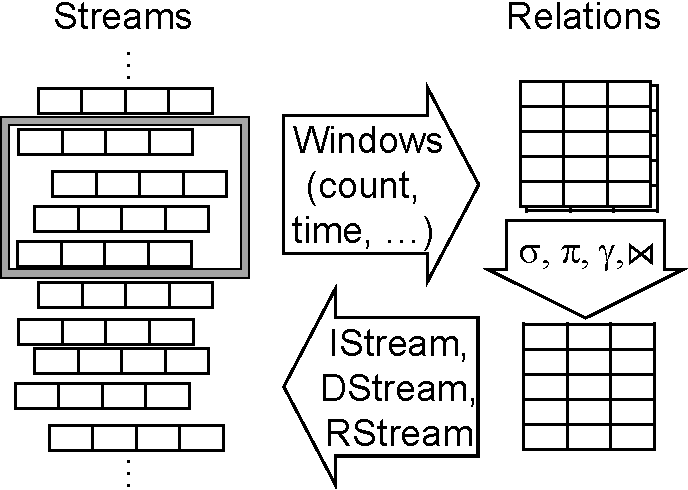
\includegraphics[scale=0.45]{cqlops.pdf}}
\vspace*{-4mm}
\caption{\label{fig:cqlops}CQL algebra operators.}
\end{figure}

In 2004, Arasu et al.\ at Stanford introduced \textsf{CQL} (for Continuous
Query Language)~\cite{arasu_widom_2004}. CQL has been designed as an
SQL-based declarative language for implementing continuous queries
against streams of data, such as the LinearRoad
benchmark~\cite{arasu_et_al_2004}. The design was influenced by the
\textsf{TelegraphCQ} system, which proposed an SQL-based language with a
focus on expressive windowing
constructs~\cite{chandrasekaran_et_al_2003}.
Dindar et al.~\cite{dindar2013modeling} presented a model to analyze  and understand the results of various window-based
queries (e.g., time- and tuple-based windows). Figure~\ref{fig:cql} illustrates a CQL code example that
uses a time-based sliding window (per minute within the last 24 hours) over
phone calls to return the maximum phone call length along with its
count and caller information.

The semantics of CQL are
based on two phases of data, \emph{streams} and \emph{relations}.
As Figure~\ref{fig:cqlops} illustrates, CQL
supports three classes of operators over these types. First,
\emph{stream-to-relation} operators freeze a stream into a relation.
These operators are based on
\emph{windows} that, at any point of time, contain a
historical snapshot of a recent portion of the stream. CQL includes
time-based and tuple-based windows, both with optional
partitioning. Second, \emph{relation-to-relation} operators, which
turn relations into another relation. These operators are expressed
using standard SQL syntax and come from traditional relational
algebra, such as select~($\sigma$), project~($\pi$),
group-by-aggregate~($\gamma$), and join~($\bowtie$).
Third, \emph{rela\-tion-to-stream} operators, which thaw a relation
back into a stream. CQL supports three operators of this class:
\texttt{IStream}, \texttt{DStream}, and \texttt{RStream} (to capture inserts, deletes, or the entire
relation).

Besides TelegraphCQ, another predecessor of CQL was
\textsf{GSQL}~\cite{cranor_et_al_2003}.  In addition to the standard SQL
operators (e.g., $\sigma$, $\pi$, $\gamma$,~$\bowtie$), GSQL supports
a \emph{merge} operator that combines streams from multiple sources in
order as specified by ordered attributes.  GSQL supports joins as long
as it can determine a window from ordered attributes and join predicates.

CQL has influenced the design of many systems, for example, \textsf{Microsoft
StreamInsight}~\cite{ali_et_al_2009} and \textsf{StreamSQL}~\cite{StreamSQL}.  Jain et al.\ described an
approach to unify two different proposed SQL extensions for
streams~\cite{jain_et_al_2008}. The first proposal, presented by
Oracle and based on CQL, used a time-based execution model that
provided a way to model simultaneity. The second proposal, presented
by \textsf{StreamBase}, used a tuple-based execution model that provided a way
to react to primitive events as soon as they are seen by the system.
Jain et al.\ captured ordering and simultaneity through partial orders
on batches of tuples using a new \emph{Spread} operator.  Zou et
al.\ showed how to turn a stream of queries into a stream query by
streaming their parameters~\cite{zou_et_al_2010}.  And Soul\'{e} et
al.~\cite{soule_et_al_2016} presented a formal type system and
small-step operational semantics for CQL via translation to a calculus
for stream processing named \texttt{Brooklet}~\cite{soule_et_al_2010}.

The design of CQL has been influenced by the temporal relational model introduced by Jensen and Sondgrass in  the early 90s~\cite{jensen1994temporal}. In this model, each temporal relation has two main dimensions: a valid time record and transaction time. Chandramouli et al.~\cite{chandramouli2012temporal} has built on top of this model by presenting \textsf{TiMR}, a framework that implements a time-oriented data processing approach using the MapReduce framework based on temporal queries.

\subsection{Synchronous Dataflow}\label{sec:sdf} % Guillaume

\begin{figure}[!h]
\begin{lstlisting}[morekeywords={node,int,bool,returns,var,when,let,tel,current}]
node tracker (speed, limit: int) returns (t: int);
var x: bool; cpt: int when x;
let
  x = (speed > limit);
  cpt = counter((0, 1) when x);
  t = current(cpt);
tel
\end{lstlisting}
\vspace*{-4mm}
\caption{\label{fig:lustre} Lustre code example.}
\end{figure}

Synchronous dataflow (SDF) languages were introduced to ease the design of
real-time embedded systems. They allow to write a well-defined
deterministic specification of the system. It is then possible to
test, verify, and generate embedded code.
The first data\-flow synchronous languages Lustre~\cite{lustre_1987}
(Caspi and Halbwachs) and Signal~\cite{signal_1991} (Le Guernic,
Benveniste, and Gautier) were proposed in France in the late 1980s.
A dataflow synchronous program is a set of equations defining streams
of values. Time proceeds by discrete logical steps, and at each step,
the program computes the value of each stream depending on its inputs
and possibly previously computed values.
This approach is reminiscent of block diagrams, a popular notation to
describe control systems.
Figure~\ref{fig:lustre} presents a Lustre code example that tracks the
number of times the speed of a vehicle exceeds the speed limit. The
counter \lstinline{cpt} starts with~$0$ and is incremented by~$1$ each
time the current speed exceed the current limit (\lstinline{when x}).
The return value \lstinline{t} maintain the last computed value
of \lstinline{cpt} between two occurrences of~\lstinline{x}
(\lstinline{current(cpt)}).

Compared to the other languages presented here, SDF languages are
relatively low level and target embedded controllers. The focus is on
compiling efficient code that executes in bounded memory with a
predictible execution time.  In particular, this imposes that the
schedule and communication rates can be statically computed by the
compiler. Additional static analyses reject programs with potential
initialization or causality issues. Compilers produce imperative code
that can be executed in a control loop without communication buffers
triggered by external events or on a periodic signal (e.g., every
millisecond). The link between logical and real time is left to the
designer of the system.

The dataflow synchronous approach has inspired
multiple languages: Lucid Synchrone~\cite{lucid_2006} combines the
dataflow synchronous approach with functional features \`a la ML,
StreamIt~\cite{streamit_2002} focuses on efficient parallel processing of large
streaming applications, and Z\'elus~\cite{zelus_2013} is a Lustre-like
language extended with ordinary differential equations to define
contin\-uous-time dynamics. Lustre is also the backbone of the
industrial language and compiler Scade~\cite{scade_2017} routinely
used to program embedded controllers in many critical applications.

\subsection{Big-Data Streaming}\label{sec:big} % Martin

\begin{figure}[!h]
\begin{lstlisting}[xleftmargin=2mm,morekeywords={stream,float64,rstring,type,int32,window,output,tuple}]
stream<float64 len, rstring caller> Calls = CallsSrc() {}
type Stat = tuple<float64 len, int32 num, rstring who>;
stream<Stat> Stats = Aggregate(Calls) {
   window Calls:sliding, time(24.0*60.0*60.0), time(60.0);
   output Stats: len = Max(Calls.len),
                 num = MaxCount(Calls.len),
                 who = ArgMax(Calls.len, Calls.caller);
}
\end{lstlisting}
\vspace*{-4mm}
\caption{\label{fig:spl}SPL code example.}
\end{figure}

The need to handle diverse data and processing requirements at scale
motivated several recent big-data streaming languages and
systems~\cite{akidau_et_al_2013,akidau_et_al_2015,carbone_et_al_2015,chandramouli_et_al_2014,hirzel_schneider_gedik_2017,kulkarni_et_al_2015,murray_et_al_2013,toshniwal_et_al_2014,zaharia_et_al_2013}.
Each of them makes it easy to integrate operators written in
general-purpose languages and to parallelize them on clusters of
multicore computers. Hirzel et al.\ introduced the \textsf{SPL}
language as part of the \textsf{IBM~Streams} product in
2010~\cite{hirzel_et_al_2009,hirzel_schneider_gedik_2017}.
Figure~\ref{fig:spl} shows an example for a similar
use-case as Figure~\ref{fig:cql}. Line~1 defines a stream
\lstinline{Calls} by invoking an operator \lstinline{CallsSrc}, and
\mbox{Lines 3-8} define a stream \lstinline{Stats} by invoking an
operator \lstinline{Aggregate}. An SPL program explicitly specifies a
directed graph of stream edges and operator nodes. Streams carry
tuples; in the examples, tuple attributes contain primitive values,
but in general, they can also contain compound values such as other
tuples or lists.  Operators create and transform streams; operators
are defined by users or libraries, not built into the
language. Operators can be further configured upon invocation, for
example, with windows or output assignments. To facilitate
distribution, SPL's semantics are defined to require minimal
synchronization between operators~\cite{soule_et_al_2016}.

\vspace*{-0.3mm}
Like SPL, the core concept of other languages for big-data streaming
is also that of a directed graph of streams and operators. This graph
is an evolution of the query plan of earlier stream-relational
systems. In fact, one can view \textsf{Aurora}~\cite{abadi_et_al_2003},
\textsf{Borealis}~\cite{abadi_et_al_2005}, and
\textsf{Spade}~\cite{gedik_et_al_2008} as the evolutionary links
between relational and big-data streaming languages. They still focused
on relational operators while already encouraging developers to
explicitly code graphs.

\vspace*{-0.3mm}
Unlike SPL, which is a stand-alone language, later big-data streaming
systems offer languages that are embedded in a general-purpose host
language, typically Java. \textsf{MillWheel} focused on key-based
partitioned parallelism and semi-automatic handling of out-of-order
data~\cite{akidau_et_al_2013}. \textsf{Naiad} focused on supporting
both streaming and iterative batch analytics~\cite{murray_et_al_2013},
using elaborate timestamps and a LINQ-based surface
language~\cite{meijer_beckman_bierman_2006}.  \textsf{Spark Streaming}
emulated streaming by repeated computations on immutable in-me\-mo\-ry
data batches~\cite{zaharia_et_al_2013}. \textsf{Storm} offered
at-least-once semantics via buffering and
acknowledgements~\cite{toshniwal_et_al_2014}.  \textsf{Trill} used
batching to improve throughput and offered an extensible
aggregation framework~\cite{chandramouli_et_al_2014}.  \textsf{Heron}
displaced Storm by adding several improvements, such as a backpressure
mechanism~\cite{kulkarni_et_al_2015}. \textsf{Beam} picks up where
MillWheel left off, giving programmers ways to reconcile event time
and processing time~\cite{akidau_et_al_2015}. And finally,
\textsf{Flink} focuses on supporting both real-time streaming and batch
analytics~\cite{carbone_et_al_2015}.

\vspace*{-0.3mm}
All of the above-listed big-data streaming systems offer embedded
languages for specifying more-or-less explicit stream graphs. An
embedded language is an advanced library or framework that makes heavy
use of host-language abstractions such as lambdas, generics, and local
variable type inference. For instance, LINQ integrates SQL-inspired
query syntax in a general-purpose
language~\cite{meijer_beckman_bierman_2006}.  Embedded languages
offer simple interoperability with their host language, as well
as leveraging host-language tools and skills~\cite{hudak_1998}. On the
downside, since they are not self-contained, they are hard to isolate
clearly from the host language, inhibiting debugging, optimization,
and standardization.

\subsection{Complex Event Processing}\label{sec:cep} % Angela

%/* Either from similar domain as CQL example:
%  alert when calls from locations over
%  10 miles apart within 60 seconds. */

\begin{figure}[!h]
\begin{lstlisting}
stream<Alert> Alerts = MatchRegex(Calls) {
  param
    partitionBy: caller;
    pattern    : ".+ tooFarTooFast";
    predicates : {
      tooFarTooFast =
            geoDist(First(loc), Last(loc)) >= 10.0
        && timeDist(First(ts), Last(ts)) <= 60.0; };
  output
    Alerts: who=caller, where=Last(loc), when=Last(ts);
}
\end{lstlisting}
\vspace*{-4mm}
\caption{\label{fig:cep}CEP example.}
\end{figure}

%/* Or from similar domain as Lustre example:
%   simple edge detector, each time a car's speed
%   increases over the speed limit, emit a tuple
%   with a count of 1. */
%stream<Edge> Edges = MatchRegex(CarUpdates) {
%  param  pattern    : "below above";
%         partitionBy: car;
%         predicates : { below = speed <= limit;
%                        above = speed > limit; };
%  output Edge: car=car, speed=Max(speed), count=1;
%}

Complex event processing (CEP) uses patterns over simple events to
detect higher-level, \emph{complex}, events that may comprise multiple
simple events.  CEP can be considered either as an alternative to
stream processing or as a special case of stream processing. The
latter consideration has led to the definition of CEP operators in
streaming languages. For example, the MatchRegex~\cite{hirzel_2012}
operator implements CEP in the library of the SPL
language~\cite{hirzel_schneider_gedik_2017} (Section~\ref{sec:big}). MatchRegex was introduced by Hirzel in~2012,
influenced by the \textsc{Match-Recognize} proposal for extending ANSI
SQL~\cite{zemke_et_al_2007}.  Compared to its SQL counterpart,
MatchRegex is simplified, syntactically concise, and easy to deploy as
a library operator. MatchRegex is implemented via code generation and
translates to an automaton for space- and time-efficient incremental
computation of aggregates. But it does not support other
functionalities beyond pattern matching, such as joins and reporting
tasks. Figure~\ref{fig:cep} shows an example for detecting a complex
event when simple phone-call events occur over 10~miles apart within
60~seconds. Line~4 defines the regular expression, where the period
(\lstinline{.}) matches any simple event; the plus (\lstinline{+})
indicates at-least-once repetition; and \lstinline{tooFarTooFast} is a
simple event defined via a predicate in \mbox{Lines 6--8}. The
\lstinline{First} and \lstinline{Last} functions reference
corresponding simple events in the overall match: in this case, the
start of the \lstinline{.+} and the simple event matched by
\lstinline{tooFarTooFast}.

In principle, there were two close predecessors of MatchRegex, namely the MATCH-RECOGNIZE~\cite{zemke_et_al_2007} clause of SQL and
SASE~\cite{WuDR06}. The former has been introduced in order to capture pattern recognition in rows of a table. Patterns are described by a regular
expression included in the PATTERN argument of the MATCH-RECOGNIZE clause and represented by variables. For instance, in our example of Figure~\ref{fig:cep}, the PATTERN argument contains a group variable given by $A+$ due to the presence of the Kleene-plus quantifier (where $A$ is defined AS
LAST(G.Loc) - FIRST(G.Loc) $\geq$ 10.0
        AND Last(T.ts) - FIRST(T.ts) $\leq$ 60.0 with $G$ and $T$ indicating the geodistance and timestamp relations). The clause permits to specify the output as a singleton (ONE ROW PER MATCH, also the default) or as a set of rows (ALL ROWS PER MATCH). The first option makes visible the columns specified in   the partition
columns, order by columns and columns defined in the MEASURES clause. For ALL
ROWS PER MATCH the visible columns include also all columns of the initial tables even though they are not used in the previous fields.
Since MATCH-RECOGNIZE is embedded in SQL, join conditions can be readily specified.

With the advent of Big Data, handling higher volumes of streaming data and being capable of accommodating larger windows become imperative. To address these two challenges, the SASE event system proposes to execute complex event queries on real-time streams.
Figure~\ref{fig:SASE} shows the high-level syntax of the language, where the first clause EVENT specifies the types of events that need to be captured, while the second clause WHERE allows to filter those events by imposing suitable predicates applied to the events attributes and the third clause WITHIN indicates a time period in a sliding window over the input stream.  The first clause also allows to specify a sequence of types of events or their non occurrence
via the special symbol $!$. However, it is not permitted to specify complex patterns under the form of regular expressions (thus with Kleene-star or Kleene-plus operator) and aggregates. Thus, the above example in Figure~\ref{fig:cep} is not expressible in SASE. The idea behind SASE is to have at disposal
a self-contained language which can be translated to suitable algebraic query expressions.

\begin{figure}[!h]
\begin{lstlisting}
EVENT ~\textit{event\_pattern}~
[WHERE ~\textit{qualification}~]
[WITHIN ~\textit{window}~]
\end{lstlisting}
\vspace*{-4mm}
\caption{\label{fig:SASE}Syntax of the Sase CEP Language.}
\end{figure}

\subsection{XML Streaming}\label{sec:xml} % Sherif

\begin{figure}[!h]
\begin{lstlisting}
CREATE ~\textit{cq\_name}~
         ~\textit{xml\_ql\_query}~
     DO ~\textit{action}~
  {START ~\textit{start\_time}~}
  {EVERY ~\textit{time\_interval}~}
  {EXPIRE ~\textit{expiration\_time}~}
\end{lstlisting}
\vspace*{-4mm}
\caption{\label{fig:Niagra}NiagaraCQ code example.}
\end{figure}

Chen et al.\ introduced NiagaraCQ~\cite{chen_et_al_2000} in 2000 as a
continuous query sub-system of the Niagara internet query engine, a
data\-base for querying distributed XML data sets developed at
University of Wisconsin and Oregon Graduate
Institute~\cite{naughton2001niagara}. NiagaraCQ implements continuous
query processing over XML files by supporting incremental evaluation
and considering only the changed portion of each updated XML file. It
supports two types of continuous queries that differ in the criteria
triggering their execution: \emph{change-based} queries, which trigger
as soon as new relevant data becomes available, and \emph{timer-based}
queries, which trigger only at specified time intervals.  NiagaraCQ is
based on XML-QL~\cite{deutsch1999query}.  It provides a command
language for creating continuous queries that follows the form
illustrated in Figure~\ref{fig:Niagra}. Using this command language,
users can implement continuous queries that combines an ordinary
XML-QL query with additional time information.  The
\textsf{\small\textit{xml\_ql\_query}} becomes effective at the
defined \textsf{\small\textit{start\_time}}.  The
\textsf{\small\textit{time\_interval}} indicates how often the query
will be executed. A query is timer-based if its
\textsf{\small\textit{time\_interval}} is non-zero; otherwise, it is
change-based.  The continuous query will be deactivated after its
\textsf{\small\textit{expiration\_time}}. The
\textsf{\small\textit{action}} triggers once the results of the XML-QL
query expression is returned.  A key optimization mechanism used in
the NiagaraCQ system is grouping the execution of similar queries to
minimize redundant work.

YFilter~\cite{diao_et_al_2002,diao2003high} implements
continuous queries based on XPath~\cite{clark_derose_1999}, also with
multi-query optimization. The main idea of YFilter is to use a single
finite state machine to represent and evaluate several XPath
expressions. In particular, YFilter exploits the commonality among path queries by merging the common prefixes
of the paths so that they are processed at most once. This  shared processing mechanism provides significant performance
improvement by avoiding redundant processing for duplicate path expressions. In order to handle value-based predicates that address contents of elements, YFilter applies two alternative approaches. The first approach approach evaluates the  predicates once the addressed elements are read from a document, while the other approach postpones predicate evaluation until the corresponding path expression has been entirely matched.

\subsection{RDF Streaming}\label{sec:rdf} % Emanuele

%\begin{alltt}TODO\scriptsize, ~0.75 pages, ~8 citations, \textcolor{red}{Emanuele, Akrivi}
%- e.g., C-SPARQL \cite{barbieri_et_al_2009}
%- stream reasoning (either separate snippet, or included here)
%\end{alltt}

In 2009, Della~Valle~et~al.~\cite{DBLP:journals/expert/ValleCHF09} called the Semantic Web and AI communities to investigate languages, tools and methodologies for representing, managing and reasoning on heterogenous data streams and complex events in presence of expressive domain models (captured by the means of ontologies). Those communities were still focusing on rather static data: knowledge bases were assumed to be static and solutions to incorporate changes were far too complex to be applicable to gigantic data streams. Della Valle et al.~\cite{DBLP:journals/expert/ValleCHF09} proposes to name this new research topic Stream Reasoning~\cite{DellAglioDataScience2017}.

\sloppy The research on Stream Reasoning investigated two parallel, but interleaved, research questions: one on modelling and one on optimisation. On the \textbf{modelling} side, early works extend the Semantic Web stack \cite{DBLP:books/daglib/0036180} in order to represent heterogenous data streams, continuous queries, and continuous reasoning tasks. Inspired by CQL~\cite{arasu_widom_2004}, Della Valle et al.~\cite{DBLP:conf/fis/ValleCBBC08} proposed the notions of RDF Stream and Continuous SPARQL (C-SPARQL). Those notions were extended in SPARQL$_{stream}$~\cite{Calbimonte2010}, CQELS~\cite{LePhuoc2012c} and EP-SPARQL~\cite{DBLP:journals/semweb/AnicicRFS12} introducing variants in syntax and semantics. Building on all those efforts an RDF Stream Processing (RSP) community group\footnote{\url{http://www.w3.org/community/rsp/}} was established at W3C in 2013  to define RSP-QL syntax~\cite{DBLP:conf/esws/DellAglioCVC15} and semantics~\cite{DBLP:journals/ijswis/DellAglioVCC14}.

In RSP-QL, an \textit{RDF Stream} is as an unbound sequence of \emph{time-varing graphs} $< t,\tau>$ where $t$ is an RDF graph and $\tau \in \mathbb{Z}^{*}$ is a non-decreasing timestamp; while a RQL-QL query is a continuous query on multiple RDF streams as well as static information stored in RDF graphs. 

Figure~\ref{fig:rdfstream} illustrates a RDF stream snippet for a similar use-case as Figure~\ref{fig:cql}. It shows two RDF graphs emitted respectively at $\tau_1$ and $\tau_2$. Each RDF graph contains a call with a caller and multiple callees. Notably, even if each call is a tree, merging multiple call results in a call graph: the two calls involve the same callee \textsf{Bob} and the caller of \textsf{call1} is a callee in  \textsf{call2}.

\begin{figure}[!h]
\begin{lstlisting}[escapeinside={(*}{*)}]
:graph1 :generatedAt "(*$\tau_1$*)"
:graph1 { 
  :call1 :caller :Alice .
  :call1 :callee :Bob .}
:graph2 :generatedAt "(*$\tau_2$*)" 
:graph2 { 
  :call2 :caller :Carl .
  :call2 :callee :Alice .
  :call2 :callee :Bob . }  
\end{lstlisting}
\vspace*{-4mm}
\caption{\label{fig:rdfstream}an RDF stream snippet.}
\end{figure}

Figure \ref{fig:rspql} illustrates an RSP-QL query that continuously identifies callee that are currently \textit{communication hubs}, i.e., they are involved in more calls than usual on this stream. Numerically, we can identify them by looking for those who in the last 30 minutes appear more frequently then in the last 2 hours. To do so, Line 1 registers a query. Lines 3-6 open on the RDF stream \textsf{in} a short window \textsf{swin} of 30 minutes that tumbles and a long window \textsf{lwin} of 120 minutes that slides every 30 minutes. Lines 8-11 and Lines 12-15 count the number of calls per callee in the long window and in short window, respectively. Line 16-17 fetche the standard deviation of the number of calls per each callee appearing in the windows from a static graph and checks if the Z-Score\footnote{\url{https://en.wikipedia.org/wiki/Standard_score}} is larger than 2. Last but not least, Line 2 declares out to emit results as a new RDF stream.

\begin{figure}[!h]
\begin{lstlisting}[language=rsp-ql]
REGISTER STREAM :out
AS CONSTRUCT RSTREAM { ?x a :Hub }
FROM NAMED WINDOW :lwin 
       ON :in [ RANGE PT120M STEP PT10M]
FROM NAMED WINDOW :swin 
       ON :in [ RANGE PT10M STEP PT10M]
WHERE { 
  WINDOW :lwin{
    SELECT ?x ( COUNT(*) AS ?totalLong)
    WHERE { ?c1 :callee ?x. }
    GROUP BY ?x }
  WINDOW :swin{
    SELECT ?x ( COUNT(*) AS ?totalShort)
    WHERE { ?c2 :callee ?x. }
    GROUP BY ?x }
  GRAPH :bg {?x :hasStandardDeviation ?s }
  FILTER ((?totalShort - ?totalLong/12)/?s > 2)
} GROUP BY ?x
\end{lstlisting}
\vspace*{-4mm}
\caption{\label{fig:rspql}RSP-QL example.}
\end{figure}

The novelty of RDF streams w.r.t. relational data streams is not in its definition, but in what it enables. When the information flow is a graph evolving over time, RDF stream data model is more adequate than relational data stream, because the same RDF stream can accommodate a variety of data elements, whereas a relational data stream allows only tuples corresponding to a defined relation to be streamed. 

\subsection{Stream Reasoning}\label{sec:rdf} % Emanuele

RDF streams also enable the encoding of continuous reasoning tasks as continuous query answering under a given entailment regime. For instance, a continuous Description Logic reasoning task~\cite{Walavalkar2008} involves 
a static TBox $T$ and a sequence of ABoxes about $T$ called
ontology stream S$^T$(i).
A windowed ontology stream S$^T$(o,c] is the unions to all the ABoxes
S$^T$(i) where $o<i\leq c$.
Figure~\ref{fig:sr} illustrates a RSP-QL query for a similar use-case as Figures~\ref{fig:cql} and~\ref{fig:rspql}. The RDF stream contains triples such as \textsf{:Alice :calls :Bob} and \textsf{:Bob :calls :Carl}. The property \textsf{:contacts} is the transitive closure of the property \textsf{:calls}. The query continuously counts the number of people \textsf{:Alice} contacts directly or indirectly through a chain of \textsf{:calls}.

\begin{figure}[!h]
\begin{lstlisting}[language=rsp-ql]
SubObjectPropertyOf( 
   ObjectPropertyChain( :calls :calls ) :contacts 
)

REGISTER STREAM ImpactMeter AS
SELECT (count(?x) AS ?impact)
FROM NAMED WINDOW :win 
       ON :in [ RANGE PT60M STEP PT10M]
WHERE { :Alice :contacts ?x }
\end{lstlisting}
\vspace*{-4mm}
\caption{\label{fig:sr}Example of RSP-QL under Description Logic entailment regime.}
\end{figure}

Reasoning over a windowed ontology stream is as reasoning in static DL, the only problem is to optimise the reasoning task in order to remain reactive. Barbieri~et~al.~\cite{DBLP:conf/esws/BarbieriBCVG10} made the first step in this direction optimising the DRed algorithm when deletion becomes predictable. Few years later Komazec~et~al.~\cite{DBLP:conf/debs/KomazecCF12} realised its first implementation extending the RETE algorithm. In parallel, Y. Ren and J. Pan proposed an alternative approach via Truth Maintenance Systems~\cite{Ren2011}. The state-of-the-art in this setting is the work of Motik~et~al.~\cite{DBLP:conf/aaai/MotikNPH15a}.  It is also worth to note that the term RDF stream denotes a data model. It does not imply that data has to be \emph{physically} represented as time-varying RDF graphs. It also allows to represent non-RDF data stream as \emph{virtual RDF streams} and to reason on it by rewriting continuous ontological queries on an underlying data stream processing system using Ontology Based Data Access principles. The state-of-the-art in this setting is the work of Calbimonte~et~al.~\cite{DBLP:conf/esws/CalbimonteMC16}.

However, alternative reasoning tasks can be performed, too. Anicic~et~al.~\cite{DBLP:journals/semweb/AnicicRFS12} bridged Stream Reasoning with Complex Event Processing grounding both in Logic Programming. Beck et al. used Answer Set Programming to model expressive Stream Reasoning tasks~\cite{DBLP:conf/aaai/BeckDEF15} and built systems able to perform those tasks, e.g.,  Ticker~\cite{DBLP:journals/tplp/BeckEB17} and Laser~\cite{DBLP:conf/semweb/BazoobandiBU17}. Inductive Stream Reasoning, i.e. applying Machine Learning techniques to RDF streams or to Ontology streams, is also an active field \cite{DBLP:conf/ijcai/ChenLPC17,DBLP:conf/ijcai/LecueP13,DBLP:journals/expert/BarbieriBCVHTRW10} .

\subsection{Streaming for End-Users}\label{sec:eup} % Martin

\begin{figure}[!h]
\centerline{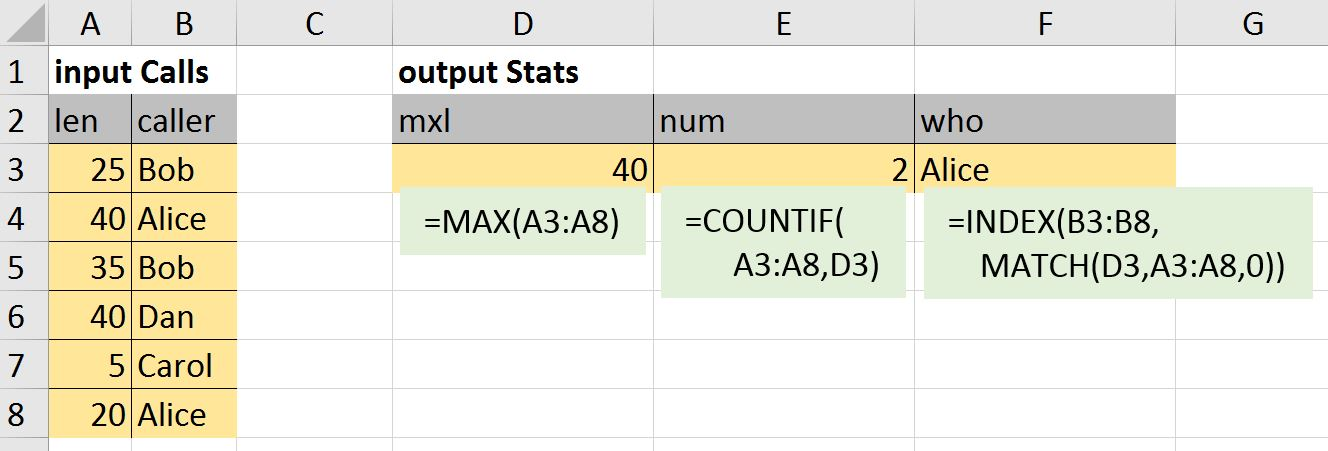
\includegraphics[width=\columnwidth]{CallStats.jpg}}
\vspace*{-4mm}
\caption{\label{fig:activesheets}ActiveSheets example.}
\end{figure}

We use the term \emph{end-users} to refer to users without particular
software development training. Probably the most successful
programming tool for end-users is spreadsheet formulas. And from the
early days of VisiCalc in 1979~\cite{bricklin_frankston_1979},
spreadsheet formulas have been \emph{reactive} in the sense that any
changes in their inputs trigger an automatic recomputation of their
outputs. Therefore, in 2014, Vaziri et al.\ designed ActiveSheets, a
spreadsheet-based stream programming model~\cite{vaziri_et_al_2014}.
Figure~\ref{fig:activesheets} gives an example that implements a
similar computation as Figures \mbox{\ref{fig:cql} and \ref{fig:spl}}.
Cells \lstinline{A3:B8} contain a sliding window of recent call
records, which ActiveSheets updates from live input data. Cells
\lstinline{D6:F6} contain the output data, \mbox{(re-)}com\-pu\-ted
using reactive spreadsheet formulas. The formula
\mbox{\lstinline{E6=COUNTIF(A3:A8,D6)}} counts how many calls in the
window are as long as a longest call. The formula
\mbox{\lstinline{F6=INDEX(B3:B8,F2)}} uses the relative index \lstinline{F2}
of the longest \lstinline{len} to retrieve the corresponding
caller.  ActiveSheets was influenced by
synchronous data\-flow~\cite{lustre_1987} and has been extended with
time-based windows, key-based partitions, and performance
optimizations~\cite{hirzel_et_al_2016}.

\begin{alltt}TODO\scriptsize
- more spreadsheets \cite{chang_myers_2015}, \cite{etzion_et_al_2016}
- trigger-action programming~\cite{ifttt}
- CNL: survey \cite{kuhn_2014}, META \cite{arnold_et_al_2016}
- search-based programming \cite{riabov_et_al_2008}
\end{alltt}

